\documentclass[journal,12pt,twocolumn]{IEEEtran}

\usepackage{setspace}
\usepackage{gensymb}
\singlespacing
\usepackage[cmex10]{amsmath}

\usepackage{amsthm}

\usepackage{mathrsfs}
\usepackage{txfonts}
\usepackage{stfloats}
\usepackage{bm}
\usepackage{cite}
\usepackage{cases}
\usepackage{subfig}

\usepackage{longtable}
\usepackage{multirow}

\usepackage{enumitem}
\usepackage{mathtools}
\usepackage{steinmetz}
\usepackage{tikz}
\usepackage{circuitikz}
\usepackage{verbatim}
\usepackage{tfrupee}
\usepackage[breaklinks=true]{hyperref}
\usepackage{graphicx}
\usepackage{tkz-euclide}

\usetikzlibrary{calc,math}
\usepackage{listings}
    \usepackage{color}                                            %%
    \usepackage{array}                                            %%
    \usepackage{longtable}                                        %%
    \usepackage{calc}                                             %%
    \usepackage{multirow}                                         %%
    \usepackage{hhline}                                           %%
    \usepackage{ifthen}                                           %%
    \usepackage{lscape}     
\usepackage{multicol}
\usepackage{chngcntr}

\DeclareMathOperator*{\Res}{Res}

\renewcommand\thesection{\arabic{section}}
\renewcommand\thesubsection{\thesection.\arabic{subsection}}
\renewcommand\thesubsubsection{\thesubsection.\arabic{subsubsection}}

\renewcommand\thesectiondis{\arabic{section}}
\renewcommand\thesubsectiondis{\thesectiondis.\arabic{subsection}}
\renewcommand\thesubsubsectiondis{\thesubsectiondis.\arabic{subsubsection}}


\hyphenation{op-tical net-works semi-conduc-tor}
\def\inputGnumericTable{}                                 %%

\lstset{
%language=C,
frame=single, 
breaklines=true,
columns=fullflexible
}
\begin{document}

\newcommand{\BEQA}{\begin{eqnarray}}
\newcommand{\EEQA}{\end{eqnarray}}
\newcommand{\define}{\stackrel{\triangle}{=}}
\bibliographystyle{IEEEtran}
\raggedbottom
\setlength{\parindent}{0pt}
\providecommand{\mbf}{\mathbf}
\providecommand{\pr}[1]{\ensuremath{\Pr\left(#1\right)}}
\providecommand{\qfunc}[1]{\ensuremath{Q\left(#1\right)}}
\providecommand{\sbrak}[1]{\ensuremath{{}\left[#1\right]}}
\providecommand{\lsbrak}[1]{\ensuremath{{}\left[#1\right.}}
\providecommand{\rsbrak}[1]{\ensuremath{{}\left.#1\right]}}
\providecommand{\brak}[1]{\ensuremath{\left(#1\right)}}
\providecommand{\lbrak}[1]{\ensuremath{\left(#1\right.}}
\providecommand{\rbrak}[1]{\ensuremath{\left.#1\right)}}
\providecommand{\cbrak}[1]{\ensuremath{\left\{#1\right\}}}
\providecommand{\lcbrak}[1]{\ensuremath{\left\{#1\right.}}
\providecommand{\rcbrak}[1]{\ensuremath{\left.#1\right\}}}
\theoremstyle{remark}
\newtheorem{rem}{Remark}
\newcommand{\sgn}{\mathop{\mathrm{sgn}}}
\providecommand{\abs}[1]{\vert#1\vert}
\providecommand{\res}[1]{\Res\displaylimits_{#1}} 
\providecommand{\norm}[1]{\lVert#1\rVert}
%\providecommand{\norm}[1]{\lVert#1\rVert}
\providecommand{\mtx}[1]{\mathbf{#1}}
\providecommand{\mean}[1]{E[ #1 ]}
\providecommand{\fourier}{\overset{\mathcal{F}}{ \rightleftharpoons}}
%\providecommand{\hilbert}{\overset{\mathcal{H}}{ \rightleftharpoons}}
\providecommand{\system}{\overset{\mathcal{H}}{ \longleftrightarrow}}
	%\newcommand{\solution}[2]{\textbf{Solution:}{#1}}
\newcommand{\solution}{\noindent \textbf{Solution: }}
\newcommand{\cosec}{\,\text{cosec}\,}
\providecommand{\dec}[2]{\ensuremath{\overset{#1}{\underset{#2}{\gtrless}}}}
\newcommand{\myvec}[1]{\ensuremath{\begin{pmatrix}#1\end{pmatrix}}}
\newcommand{\mydet}[1]{\ensuremath{\begin{vmatrix}#1\end{vmatrix}}}
\numberwithin{equation}{subsection}
\makeatletter
\@addtoreset{figure}{problem}
\makeatother
\let\StandardTheFigure\thefigure
\let\vec\mathbf
\renewcommand{\thefigure}{\theproblem}
\def\putbox#1#2#3{\makebox[0in][l]{\makebox[#1][l]{}\raisebox{\baselineskip}[0in][0in]{\raisebox{#2}[0in][0in]{#3}}}}
     \def\rightbox#1{\makebox[0in][r]{#1}}
     \def\centbox#1{\makebox[0in]{#1}}
     \def\topbox#1{\raisebox{-\baselineskip}[0in][0in]{#1}}
     \def\midbox#1{\raisebox{-0.5\baselineskip}[0in][0in]{#1}}
\vspace{3cm}
\title{AI1103-Assignment 2}
\author{Name : Ayush Jha \\ Roll Number: CS20BTECH11006}
\maketitle
\newpage
\bigskip
\renewcommand{\thefigure}{\theenumi}
\renewcommand{\thetable}{\theenumi}
Download all python codes from 
\begin{lstlisting}
https://github.com/ayushjha2612/AI11003/tree/main/Assignment2/Codes
\end{lstlisting}
%
and latex-tikz codes from 
%
\begin{lstlisting}
https://github.com/ayushjha2612/AI11003/tree/main/Assignment2
\end{lstlisting}
\section*{Problem 5.27}
Find the probability distribution of number of doublets in three throws of a pair of dice?
\section*{Solution}
Let $X1, X2 \in \{1, 2, 3, 4, 5, 6\}$ represent the two dice.
We have,
$$\Pr\brak{X_1 =X_2} = \frac{6}{36} = \frac{1}{6}$$
Similarly we have, 
$$\Pr\brak{X_1 \neq X_2} = \frac{30}{36} = \frac{5}{6}$$
Let the number of doublets in three throws of a pair of dice be represented by a random variable, $X$ \\
When a pair of dice is thrown three times the number of doublets can be 0,1,2 and 3 respectively. So X can take these values
\begin{align}
    \Pr\brak{X =0} &= {\Pr\brak{X_1 \neq X_2}}^3   \\
        &=  \frac{5}{6} \times \frac{5}{6} \times \frac{5}{6} \\
        & = \frac{125}{216} \\
        & = 0.5787
\end{align}
Similarly we have, 
\begin{align}
    \Pr\brak{X =1} &= 3 \times {\Pr\brak{X_1 \neq X_2}}^2 \times \Pr\brak{X_1 = X_2}   \\
        &=  3\times \frac{5}{6} \times \frac{5}{6} \times \frac{1}{6} \\
        & = \frac{75}{216} \\
        & = 0.34722
\end{align}
\textbf{Note :} 3 is multiplied as we have to select which dice will have doublet
\begin{align}
    \Pr\brak{X =2} &= 3 \times \Pr\brak{X_1 \neq X_2} \times {\Pr\brak{X_1 = X_2}}^2 \\
        &=  3\times \frac{5}{6} \times \frac{1}{6} \times \frac{1}{6} \\
        & = \frac{15}{216} \\
        & = 0.06944
\end{align}
And lastly,
\begin{align}
    \Pr\brak{X =2} &= {\Pr\brak{X_1 = X_2}}^3   \\
        &=   \frac{1}{6} \times \frac{1}{6} \times \frac{1}{6} \\
        & = \frac{1}{216} \\
        & = 0.00463
\end{align}
The probability distribution of number of doublets in three throws of a pair of dice can be found out at figure \ref{Probability distribution}. 
\begin{figure}[h!]
    \centering
    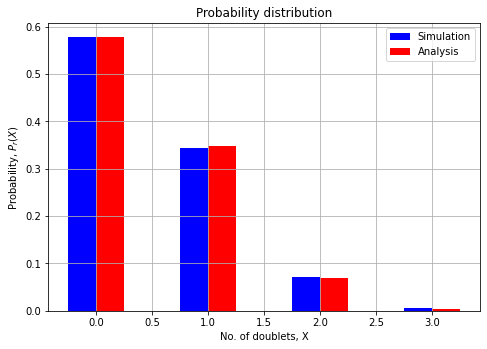
\includegraphics[width=11cm]{Assignment_2.png}
    \caption{Probability distribution}
    \label{Probability distribution}
\end{figure}
\end{document}